\section{Experimental Results}
We conduct experiments on three datasets, where each dataset is obtained by monitoring the 24-hour activities of two adults in a house via RFID. 
All these activities occur in twelve rooms; the house's basement, bathroom, bedroom, dining room, hallway, kitchen, living room, mudroom, nursery, outside-front, outside-back, and upstairs.  
\begin{table}[h]
\caption{Datasets summary.} 
\label{tab_dataset}
\centering
\begin{tabular} {|c|c|c|c|}
\hline
Dataset & Number of entries & Period(day) & Start date\\
\hline
study 10  & 6596 & 12 & 02/10/2014\\
\hline
study 11  & 1696 & 10 & 01/29/2014\\
\hline
study 14 & 3453 & 13 & 12/09/2013\\
\hline
\end{tabular}
\end{table}
The dataset comprises a set of events in the form of timestamped room occupancy data points. For instance, an event can correspond to person 1 being in the kitchen at 7:00 am. The three datasets are summarized in Table~\ref{tab_dataset}.
Here, \textit{unoccupancy} of a person is defined as one of the following conditions: the person has left the {\em outside-front} or {\em outside-back} of the house for more than 30 minutes; the person has remained in the living room or dining room for more than 9 hours with no other activities; or the gap between any two events is more than 30 minutes. 
Since our research goal is to automate switching the HVAC system on or off at least 30 minutes before a change in occupancy occurs, the first and third constraints are in place. We are only interested in events where the {\em unocupancy} period is for an extended duration ($>$ 30 minutes). The second constraint comes from our observation that if a person appears to remain in the same room for more than 9 hours without moving to another room, 
this usually means that that person has gone out but left the RFID equipment at home. 
We also delete events with a duration of less than 
2 minutes since these correspond to the individual walking back and forth across rooms and generally do not contribute to meaningful episodes. We conduct four types of experiments to compare the four approaches; 
kNN, mixture EGH, PDF, and support vector regression (SVR). 
For each dataset, we use $2/3$ of the data for training and the remaining $1/3$ of the data as the test set. 
Following the approach in~\cite{scott2011preheat},
we organize each day's data into 96 15-minute periods. 
For the test data, we assume that we only know some of the 15-minute periods. Our target is thus to predict the occupancy for the reminder of the day, or for 30 minutes ahead. 

\subsection{Occupancy Prediction for Individuals}
\begin{table*}[t]
%\vspace{0.2cm}
\hfill
%\begin{minipage}[t]{1.0\linewidth}%

\caption{Precision Recall F-measure Comparison of Individual and Whole House Occupancy Prediction in Study 14.}
\label{tab_individualResults}
%\tbl{Precision Recall F-measure Comparison of Individual and Whole House Occupancy Prediction in Study 14.\label{tab_individualResults}}{
%\begin{center}
%\makebox[\textwidth]{
\centering
\small
\setlength\tabcolsep{2pt}
\begin{tabular} {|l|l|l|l|l|l|l|l|l|l|l|l|l|l|l|l|}
\hline
\multirow{2}{*}{Dataset}&\multirow{2}{*}{Date}&\multirow{2}{*}{Person} & \multicolumn{3}{|c|}{EGH}&\multicolumn{3}{|c|}{kNN} &\multicolumn{3}{|c|}{SVM}   \\
\cline{4-12}
&&& precision & recall &fmeasure &precision & recall & fmeasure &precision & recall & fmeasure \\
\hline
\multirow{3}{*}{study10}  & 02/17/2014 & person2& \textbf{1.00} & \textbf{1.00}&\textbf{1.00} & 0.99 & 0.98 & 0.98 &0.71 &0.76 & 0.71\\
\cline{2-12}
& 02/19/2014 & person1& 0.98 & 0.99 &0.98&  \textbf{0.99} &  \textbf{0.99} &  \textbf{0.99} & 0.71 & 0.76 & 0.70 \\
\cline{2-12}
& 02/20/2014 & person2&  \textbf{0.93} &  \textbf{0.92} &  \textbf{0.92} & 0.92 & 0.91 & 0.90 & 0.72 & 0.77 & 0.72\\
\cline{2-12}
& 02/20/2014 & person1&  \textbf{0.95}& \textbf{0.94} & \textbf{0.94} & 0.94	& 0.93 & 0.93 & 0.71 & 0.77 & 0.72 \\
\cline{2-12}
& 02/20/2014 & \textbf{wholehouse}&  \textbf{0.92}& \textbf{0.92} & \textbf{0.91} & 0.91	& 0.89 & 0.91 & 0.79 & 0.74 & 0.74 \\
\hline
\hline
\multirow{3}{*}{study11}  & 02/04/2014 & person2& 0.93 & 0.93 & 0.92  & \textbf{0.95} & \textbf{0.95} & \textbf{0.95} & 0.71 & 0.77 &0.72\\
\cline{2-12}
& 02/04/2014 & person1& 0.93 & 0.93 & 0.92  & \textbf{0.95} & \textbf{0.95} & \textbf{0.95} & 0.70 & 0.77 & 0.71  \\
\cline{2-12}
& 02/05/2014 & person2&  \textbf{0.85} &  \textbf{0.92} &  \textbf{0.86} & 0.87 & 0.87 & 0.84 & 0.71 & 0.76 & 0.71 \\
\cline{2-12}
& 02/05/2014 & person1&  \textbf{0.84} &  \textbf{0.90} &  \textbf{0.84} & 0.79 & 0.90 & 0.80  & 0.70 & 0.77 & 0.71   \\
\cline{2-12}
& 02/04/2014 & \textbf{wholehouse}&  \textbf{0.918}& \textbf{0.924} & \textbf{0.913} & 0.916	& 0.921 & 0.911 & 0.77 & 0.69 & 0.71  \\
\cline{2-12}
& 02/05/2014 & \textbf{wholehouse}&  \textbf{0.90}& \textbf{0.84} & \textbf{0.84} & 0.88	& 0.81 & 0.81 & 0.74 & 0.70 & 0.70\\
\hline
\end{tabular}
%}
%\end{center}
%\end{minipage}%
%\hfill%
\end{table*}
The individual occupancy prediction results for the datasets Study 10 and Study 11 are summarized in Table~\ref{tab_individualResults}. 
In Study 10,  the mixture EGH performs better than kNN for the occupancy prediction for person 2 on 02/17/2014. 
The mixture EGH also outperforms kNN for both subjects on 02/20/2014. 
However, for person 1 on 02/19/2014, kNN works slightly better. 
When checking the original data for the test date, 
we discover that the activities on this date were very similar to the historical activities in the training data, 
%\textbf{When checking the original data, we find that the date on that day is similar to the historical data. - need to rephrase}
which leads us to the conclude that when the test data is highly similar to the historical data, 
the kNN approach may perform a little better.  
In the Study 11, mixture EGH achieves higher precision, recall and f-measure scores on 02/05/2014, but not on 02/04/2014. 
We again analyze the original data to find the reason for kNN's better performance, and find a deviation from the normal pattern, since both individuals went to sleep later than usual that day (after 12:00am).
Also, before they went to sleep, person 1 stayed in the kitchen for around two hours. 
The frequent episode $KZ$, which represents 'kitchen-unoccupied', 
usually occurs in the morning instead of around midnight. 
However, the mixture EGH model still assumes that the $KZ$ pattern 
occurred during the morning, so the prediction results are not accurate in this case. 
%\textbf{On the contrary, 
%kNN doesn't consider the 
%actual place inside the room. - need to rephrase}
Since kNN ignores this fine granular activity pattern in the household and only considers the occupancy status 
over the previous five most similar days, its performance is better. 
Generally speaking, the mixture EGH helps predict when a person 
would leave home and his/her sleep period, delivering a  
performance comparable to that achieved using the kNN approach. 
For all these experiments, the SVR approach performs the worst because 
of the limitations of this approach. 
SVR uses several of the most recent data points for the occupancy state as the 
training vector for the prediction of the next occupancy state. 
Here we set eight past data points as the predictor, but
other features such as the time of day and day of week can not be utilized fully. 

We also conduct experiments to predict the participants' {\em rest-of-day} occupancy at different times. 
\begin{figure}[h]
\centering
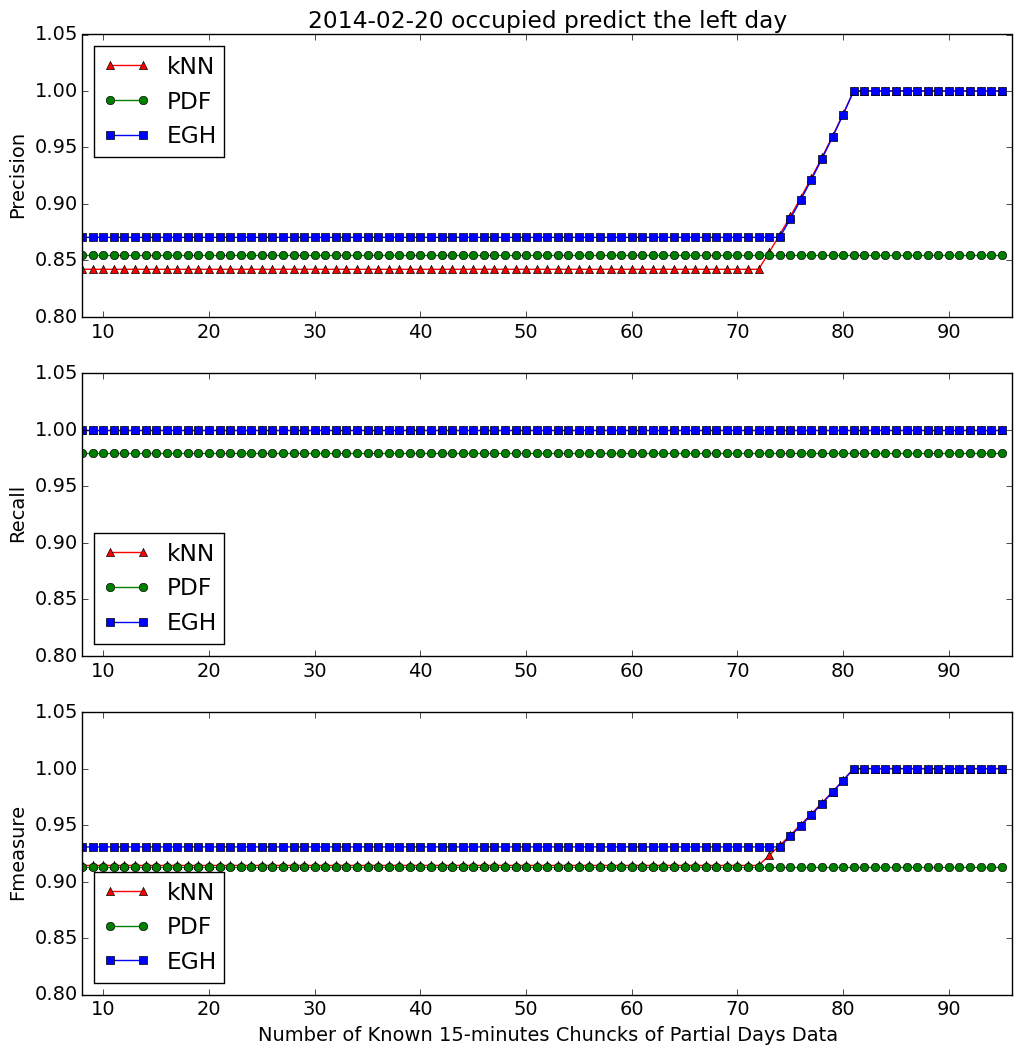
\includegraphics[width=0.5\textwidth]{adlfigs/study10person12014-02-20occupied.png}
\caption{Occupancy prediction precision, recall and f-measure comparison of three approaches 
of person 1 on 02/20/2014 on Study 10.}
\label{fig_study10}
\end{figure}
Figure~\ref{fig_study10} illustrates a person's occupancy prediction result from Study 10.
There are three sub-figures, with 
each sub-figure describing the 
precision, recall, and f-measure 
for person 1 on 02/20/2014. 
The blue line represents the mixture EGH model,
the green line represents the PDF model,
and the red line denotes the kNN model. 
The x-axis is the number of known 15-minute periods for the test day. 
For instance, at $x=20$, 
we already know $20*15$ minutes' data 
and need to predict whether the home will be occupied during the remaining $76$ time periods. 
The y-axis denotes the precision, recall and f-measure values 
in the three sub-figures from the top down. 
The first sub-figure shows that mixture EGH has the highest precision, recall and f-measure on test day 02/20/2014 
for occupancy prediction. The other two baseline approaches are comparable, except that kNN performs better than PDF 
when the person returned home after slot 72. 
Looking at the original data, we find that person 1 actually came home later than usual 
in the data used for the training dataset. 

\iffalse
Figure~\ref{fig_study14} (a) and (b) describe the case of person1 on 12/18/2013. 
Similar to Figure \ref{fig_study11} (a) and (b), 
mixture EGH model doesn't perform well before the person1 gets up 
and the reason keeps the same. 
The person 1 slept late and some confused episodes are generated. 
Figure \ref{fig_study14} (c) and (d) describe the case of person1 on 12/19/2013. 
kNN performs better. MixtureEGH doesn't perform well because 12/19, 02/20 the person went out again after coming back and staying home for some time. However the training data don't include such case. 
\begin{figure}[h]
\centering
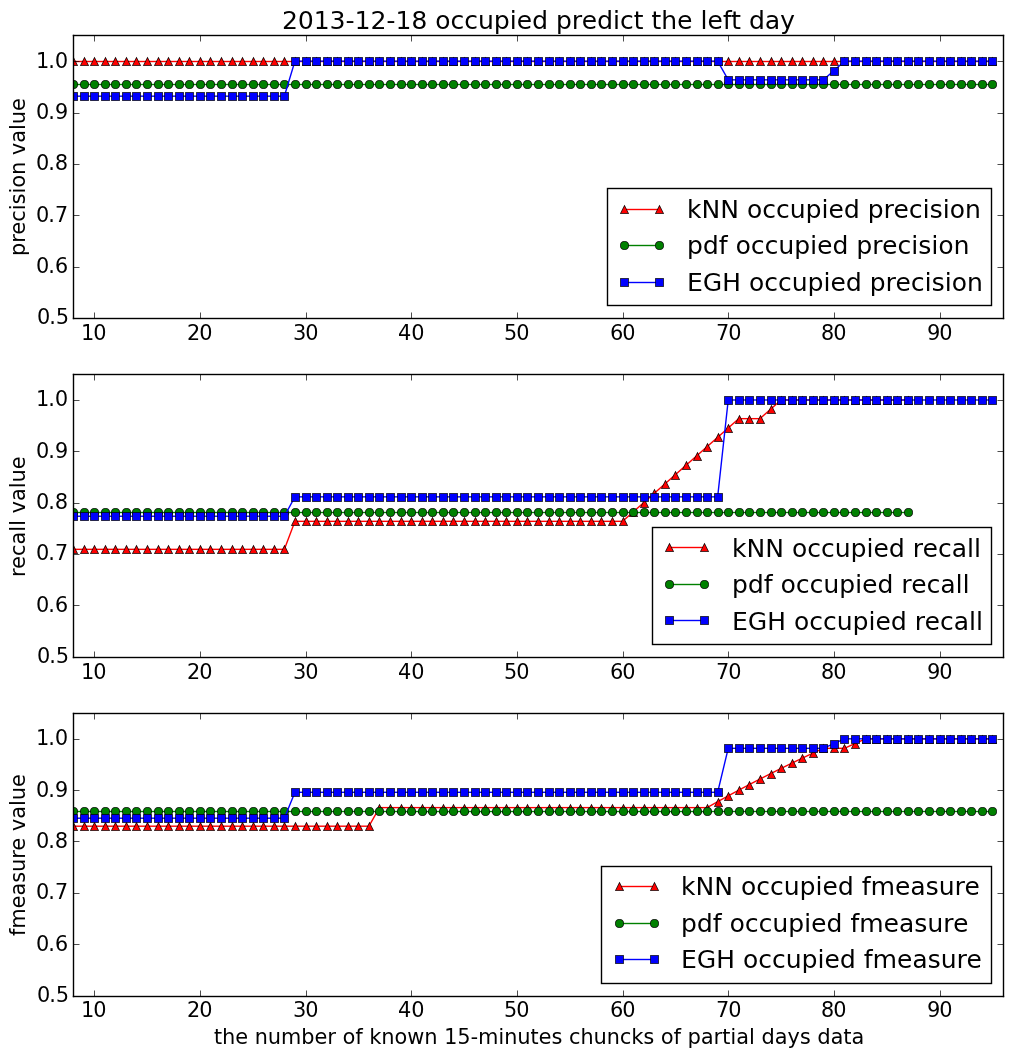
\includegraphics[width=0.5\textwidth]{adlfigs/study14person12013-12-18occupied.png} 
\caption{Study 14 Precision recall and f-measure comparison of three approaches.
person 1 occupied 12/18/2014.}
\label{fig_study14}
\end{figure}
\fi


\subsection{Occupancy Prediction of Residential Buildings}
Based on the individual prediction results, we go on to deduce when the house will be occupied
using logic OR operations on the prediction results for the two study participants. 
The whole house occupancy prediction results are listed in 
Table~\ref{tab_individualResults} and marked in bold. 
In Study 10, the precision, recall, and fmeasure values of the whole house are 0.92, 0.92 and 0.91, respectively,  
higher than the values from either the kNN approach of 0.91, 0.90 and 0.91, or the SVR approach's 0.79, 0.74 and 0.74. 
Similarly, the mixture EGH model outperforms kNN in Study 11. 
However, it is important to note that in Study 11 on 02/04/2015, 
EGH does not perform as well as kNN on individuals
but performs a little bit better than kNN, and much better than SVR, 
for the occupancy prediction for the whole house. 
This is likely because the activities of the two people inside the home 
were not synchronized. The mixture EGH model is able to predict the 
occupancy for each person and capture each person's activities more accurately. 
%When applying the logic OR operations on these two persons, 
%for whole-house occupancy prediction. 
\subsection{Limitations of Mixture EGH Model}
Although the temporal mixture EGH model performs well on the datasets Study 10 and Study 11, 
the same cannot be said for the dataset Study 14. 
Table~\ref{tab_resultsLimitation} shows that 
in Study 14, 
the mixture EGH model performs better for the individual and whole-house occupancy predictions on 12/18/2013 but not on either 12/19/2013 or 12/20/2013. 
Checking the activities of the study participants on these two days, 
we find that both went out again 
after coming back and staying home for a while.
Since the episodes of going out again after returning home from work 
do not occur frequently, the mixture EGH is unable to detect this pattern. 
Thus, the occupancy prediction probability for these events 
is completely absent. However, kNN performs well for such events because it leverages all the 
historical data and so if an abnormal event occurs just once, 
this prediction approach incorporates it when calculating the average value. 
To relax the limitations for abnormal events, 
we therefore propose a hybrid model for prediction:
when deploying this occupancy prediction, 
for example for a prediction that is 30 minutes ahead, 
just 15 minutes before the prediction, if a person goes out again after coming back, 
the deployed system switches to the kNN approach rather than the mixture EGH model for the prediction. 
In such cases, this hybrid model should always yield the best prediction results. 

\begin{table*}[!t]
%\vspace{0.2cm}
\hfill
%\begin{minipage}[t]{1.0\linewidth}%

\caption{Precision Recall F-measure of Individual and Whole House Occupancy Prediction in Study 14.}
\label{tab_resultsLimitation}
%\tbl{Precision Recall F-measure of Individual and Whole House Occupancy Prediction in Study 14.\label{tab_resultsLimitation}}{
%\begin{center}
%\makebox[\textwidth]{
\centering
\small
\setlength\tabcolsep{2pt}
\begin{tabular} {|l|l|l|l|l|l|l|l|l|l|l|l|}
\hline
\multirow{2}{*}{Dataset}&\multirow{2}{*}{Date}&\multirow{2}{*}{Person} & \multicolumn{3}{|c|}{EGH}&\multicolumn{3}{|c|}{kNN} & \multicolumn{3}{|c|}{SVM} \\
\cline{4-12}
&&& precision & recall &fmeasure &precision & recall & fmeasure &precision & recall & fmeasure  \\
\hline
\multirow{3}{*}{study14}  & 12/18/2013 & person2&  \textbf{0.91} &  \textbf{0.91} &  \textbf{0.89} & 0.87 & 0.87 & 0.84 & 0.73 & 0.77 & 0.71\\
\cline{2-12}
& 12/18/2013 & person1&  \textbf{0.92} &  \textbf{0.92} &  \textbf{0.91} & 0.90 & 0.90 & 0.89 & 0.73 & 0.76 & 0.71 \\
\cline{2-12}
& 12/19/2014 & person2& 0.86 & 0.86 & 0.85  & \textbf{0.90} & \textbf{0.90} & \textbf{0.88} & 0.73 & 0.76 & 0.71\\
\cline{2-12}
& 12/19/2014 & person1& 0.85 & 0.84 & 0.84  & \textbf{0.86} & \textbf{0.86} & \textbf{0.85} & 0.73 & 0.76 & 0.71 \\
\cline{2-12}
& 12/20/2014 & person2& 0.92 & 0.94 & 0.92  & \textbf{0.98} & \textbf{0.97} & \textbf{0.97} & 0.75 & 0.79 & 0.75 \\
\cline{2-12}
& 12/20/2014 & person1& 0.90 & 0.91 & 0.90  & \textbf{0.95} & \textbf{0.95} & \textbf{0.95} & 0.75 & 0.79 & 0.75\\
\cline{2-12}
& 12/18/2013 & \textbf{wholehouse}&  \textbf{0.91}& \textbf{0.91} & \textbf{0.90} & 0.88	& 0.88 & 0.86 & 0.75 & 0.72 & 0.70 \\
\cline{2-12}
& 12/19/2013 & \textbf{wholehouse} & 0.841	& 0.845 & 0.838&  \textbf{0.848}& \textbf{0.853} & \textbf{0.842} & 0.79 & 0.74 & 0.74 \\
\cline{2-12}
& 12/20/2013 & \textbf{wholehouse} & 0.92	& 0.90 & 0.90&  \textbf{0.94}& \textbf{0.93} & \textbf{0.93} & 0.74 & 0.72 & 0.70 \\
\hline
\end{tabular}
%}
%\end{center}
%\end{minipage}%
%\hfill%
\end{table*}
\subsection{House Occupancy Prediction 30 Minutes Ahead with Hybrid Approach}
To adequately preheat the house prior to the occupants' return, 
we need to evaluate how much time to allow in advance to automatically turn on/off the HVAC. 
Here, the advance notice time estimate given in~\cite{scott2011preheat} is utilized 
and a prediction time of 30 minutes ahead of house occupancy applied. 
%because it is reasonable for preheating. 
We compare the receiver operating characteristic (ROC curve) of three approaches: 
the mixture EGH model,  kNN, and a hybrid approach consisting of the mixture EGH model plus kNN. 
In this hybrid approach, 
we set the mixture EGH results as the baseline, 
but replace the values of the mixture model with the values obtained from the kNN model 
in the following two situations: 
1) after a person returns home; and 2) when the prediction probability of kNN is greater than 0.8. 
Figures~\ref{fig_rocresults_1}, ~\ref{fig_rocresults_2}, and~\ref{fig_rocresults_3} illustrate the ROC curve for the whole house occupancy prediction on 02/20/2014 for the dataset Study 10, 02/04/2014 for the dataset Study 11 
and 12/20/2013 for the dataset Study 14, respectively.  
The red and green lines represent the kNN and mixture EGH models; 
the blue line denotes the hybrid approach. 
The ROC curves show that the hybrid approach consistently produces the largest areas for the three cases, 
namely 
0.96, 0.92 and 0.92, respectively, 
which indicate that the hybrid approach always performs best. 
%\begin{figure}[h]
	\centering{
		\begin{tabular}{cccc}		
		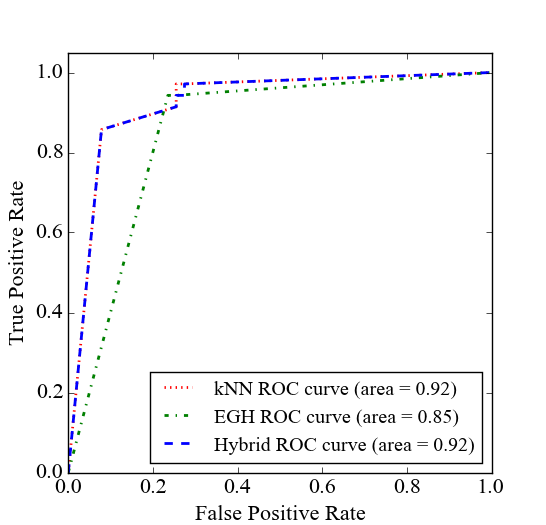
\includegraphics[width=0.5\textwidth]{adlfigs/study10ROC_02202014.png} &
		\tabular newline
		(a)\tabularnewline
		\end{tabular}
		}
	\caption{
	ROC curve of house occupancy prediction in Study10 (02/20/2014).}
	\label{fig_rocresults_1}
\end{figure}

\begin{figure}[h]
	\centering{
		\begin{tabular}{cccc}		
		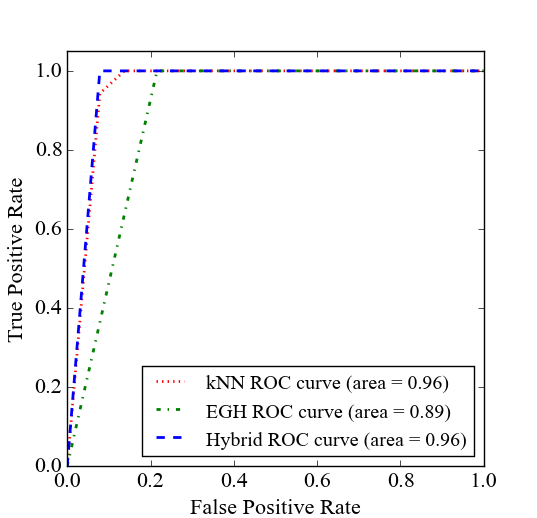
\includegraphics[width=0.5\textwidth]{adlfigs/study11ROC_02042014.png} &
		\tabularnewline
		((b)\tabularnewline
		\end{tabular}
		}
	\caption{
	ROC curve of house occupancy prediction in Study11 (02/04/2014).
}
	\label{fig_rocresults_2}
\end{figure}

\begin{figure}[h]
	\centering{
		\begin{tabular}{cccc}		
		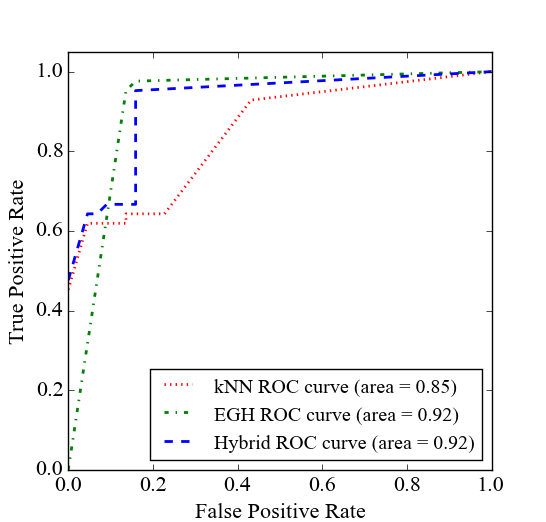
\includegraphics[width=0.5\textwidth]{adlfigs/study14ROC_12202013.png}
		\tabularnewline
		(c) \tabularnewline
		\end{tabular}
		}
	\caption{
	ROC curve of house occupancy prediction in (c) Study14 (12/20/2013).
}
	\label{fig_rocresults_3}
\end{figure}
\begin{figure}[h]
	\centering{
		\begin{tabular}{cccc}		
		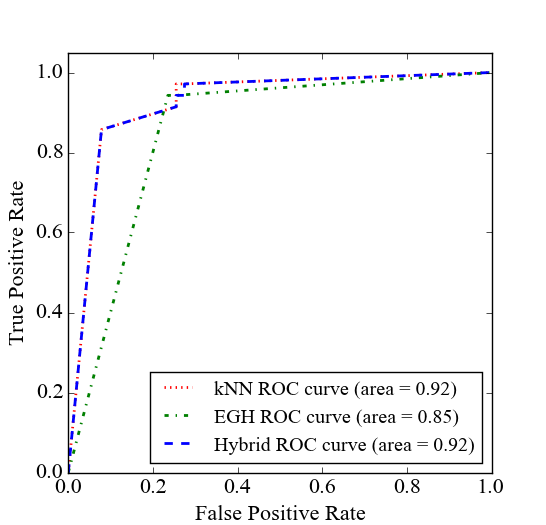
\includegraphics[width=0.5\textwidth]{adlfigs/study10ROC_02202014.png} &
		\tabularnewline
		(a)\tabularnewline
		\end{tabular}
		}
	\caption{
	ROC curve of house occupancy prediction in Study 10 (02/20/2014).}
	\label{fig_rocresults_1}
\end{figure}

\begin{figure}[h]
	\centering{
		\begin{tabular}{cccc}		
		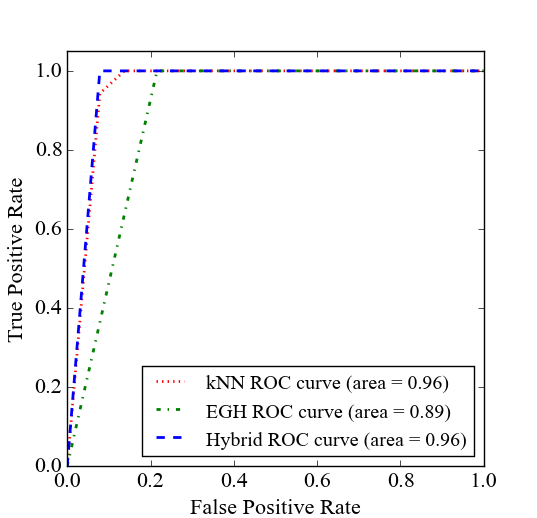
\includegraphics[width=0.5\textwidth]{adlfigs/study11ROC_02042014.png} &
		\tabularnewline
		((b)\tabularnewline
		\end{tabular}
		}
	\caption{
	ROC curve of house occupancy prediction in Study 11 (02/04/2014).
}
	\label{fig_rocresults_2}
\end{figure}

\begin{figure}[h]
	\centering{
		\begin{tabular}{cccc}		
		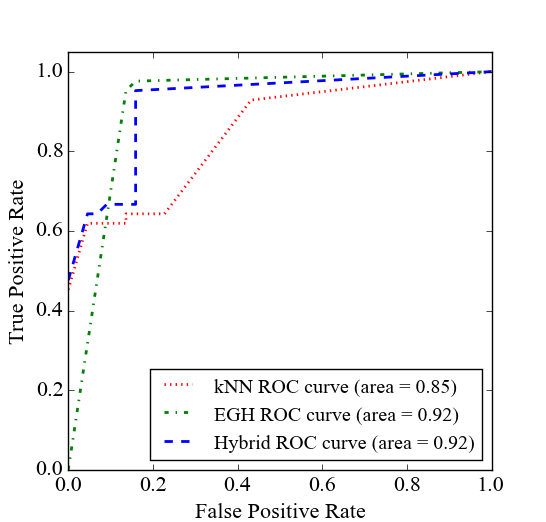
\includegraphics[width=0.5\textwidth]{adlfigs/study14ROC_12202013.png}
		\tabularnewline
		(c) \tabularnewline
		\end{tabular}
		}
	\caption{
	ROC curve of house occupancy prediction in (c) Study 14 (12/20/2013).
}
	\label{fig_rocresults_3}
\end{figure}



